

%----------------------------------------------------------------------------------------
%	PACKAGES AND OTHER DOCUMENT CONFIGURATIONS
%----------------------------------------------------------------------------------------

\documentclass{article}

\usepackage{fancyhdr} % Required for custom headers
\usepackage{lastpage} % Required to determine the last page for the footer
\usepackage{extramarks} % Required for headers and footers
\usepackage[usenames,dvipsnames]{color} % Required for custom colors
\usepackage{graphicx} % Required to insert images
\usepackage{listings} % Required for insertion of code
\usepackage{courier} % Required for the courier font
\usepackage[table]{xcolor}
\usepackage{multirow}
\usepackage{tabularx}
\usepackage{hyperref}
\usepackage{algorithm}
\usepackage{algpseudocode} 

% Margins
\topmargin=-0.45in
\evensidemargin=0in
\oddsidemargin=0in
\textwidth=6.5in
\textheight=9.0in
\headsep=0.25in

\linespread{1.1} % Line spacing

% Set up the header and footer
\pagestyle{fancy}
\lhead{\hmwkAuthorName\ : \hmwkStudentID} % Top left header
\chead{ \hmwkClassShort} % Top center head
\rhead{\firstxmark } % Top right header
\lfoot{\lastxmark} % Bottom left footer
\cfoot{} % Bottom center footer
\rfoot{Page\ \thepage\ of\ \protect\pageref{LastPage}} % Bottom right footer
\renewcommand\headrulewidth{0.4pt} % Size of the header rule
\renewcommand\footrulewidth{0.4pt} % Size of the footer rule

\setlength\parindent{0pt} % Removes all indentation from paragraphs

%----------------------------------------------------------------------------------------
%	CODE INCLUSION CONFIGURATION
%----------------------------------------------------------------------------------------

\definecolor{MyDarkGreen}{rgb}{0.0,0.4,0.0} % This is the color used for comments
\lstloadlanguages{C} % Load Perl syntax for listings, for a list of other languages supported see: ftp://ftp.tex.ac.uk/tex-archive/macros/latex/contrib/listings/listings.pdf
\lstset{language=C, % Use c in this example
        frame=single, % Single frame around code
        basicstyle=\small\ttfamily, % Use small true type font
        keywordstyle=[1]\color{Blue}\bf, % cfunctions bold and blue
        keywordstyle=[2]\color{Purple}, % c function arguments purple
        keywordstyle=[3]\color{Blue}\underbar, % Custom functions underlined and blue
        identifierstyle=, % Nothing special about identifiers                                         
        commentstyle=\usefont{T1}{pcr}{m}{sl}\color{MyDarkGreen}\small, % Comments small dark green courier font
        stringstyle=\color{Purple}, % Strings are purple
        showstringspaces=false, % Don't put marks in string spaces
        tabsize=5, % 5 spaces per tab
        %
        % Put standard c functions not included in the default language here
        morekeywords={rand},
        %
        % Put c function parameters here
        morekeywords=[2]{on, off, interp},
        %
        % Put user defined functions here
        morekeywords=[3]{test},
       	%
        morecomment=[l][\color{Blue}]{...}, % Line continuation (...) like blue comment
        numbers=left, % Line numbers on left
        firstnumber=1, % Line numbers start with line 1
        numberstyle=\tiny\color{Blue}, % Line numbers are blue and small
        stepnumber=1 % Line numbers go in steps of 5
}

% Creates a new command to include a script, the first parameter is the filename of the script (without .txt), the second parameter is the caption
\newcommand{\Cscript}[2]{
\begin{itemize}
\item[]\lstinputlisting[caption=#2,label=#1]{#1.txt}
\end{itemize}
}
\renewcommand{\arraystretch}{1.5}

%----------------------------------------------------------------------------------------
%	DOCUMENT STRUCTURE COMMANDS
%	Skip this unless you know what you're doing
%----------------------------------------------------------------------------------------

% Header and footer for when a page split occurs within a problem environment
\newcommand{\tab}[1]{\hspace{.08\textwidth}{#1}}
\newcommand{\enterProblemHeader}[1]{
\nobreak\extramarks{#1}{#1 continued on next page\ldots}\nobreak
\nobreak\extramarks{#1 }{#1 continued on next page\ldots}\nobreak
}

% Header and footer for when a page split occurs between problem environments
\newcommand{\exitProblemHeader}[1]{
\nobreak\extramarks{#1}{#1 continued on next page\ldots}\nobreak
\nobreak\extramarks{#1}{}\nobreak
}

\setcounter{secnumdepth}{0} % Removes default section numbers
\newcounter{homeworkProblemCounter} % Creates a counter to keep track of the number of problems

\newcommand{\homeworkProblemName}{}
\newenvironment{homeworkProblem}[1][Problem \arabic{homeworkProblemCounter}]{ % Makes a new environment called homeworkProblem which takes 1 argument (custom name) but the default is "Problem #"
\stepcounter{homeworkProblemCounter} % Increase counter for number of problems
\renewcommand{\homeworkProblemName}{#1} % Assign \homeworkProblemName the name of the problem
\section{\homeworkProblemName} % Make a section in the document with the custom problem count
\enterProblemHeader{\homeworkProblemName} % Header and footer within the environment
}{
\exitProblemHeader{\homeworkProblemName} % Header and footer after the environment
}

\newcommand{\problemAnswer}[1]{ % Defines the problem answer command with the content as the only argument
\noindent\framebox[\columnwidth][c]{\begin{minipage}{0.98\columnwidth}#1\end{minipage}} % Makes the box around the problem answer and puts the content inside
}

\newcommand{\homeworkSectionName}{}
\newenvironment{homeworkSection}[1]{ % New environment for sections within homework problems, takes 1 argument - the name of the section
\renewcommand{\homeworkSectionName}{#1} % Assign \homeworkSectionName to the name of the section from the environment argument
\subsection{\homeworkSectionName} % Make a subsection with the custom name of the subsection
\enterProblemHeader{\homeworkProblemName} % Header and footer within the environment
}{
\enterProblemHeader{\homeworkProblemName} % Header and footer after the environment
}

%----------------------------------------------------------------------------------------
%	NAME AND CLASS SECTION
%----------------------------------------------------------------------------------------

\newcommand{\hmwkTitle}{210CT - Programming, Algorithms \\and Data Structures\\ Coursework} % Assignment title
\newcommand{\hmwkDueDate}{March 20th 2015} % Due date
\newcommand{\hmwkClass}{ECU178 \- Computer Science} % Course/class
\newcommand{\hmwkClassTime}{10:30am} % Class/lecture time
\newcommand{\hmwkClassInstructor}{} % Teacher/lecturer
\newcommand{\hmwkAuthorName}{Robert Rigler} % Your name
\newcommand{\hmwkStudentID}{4939377}% My Student ID
\newcommand{\hmwkClassShort}{210CT Coursework } %Short name for class (only used in header)

%----------------------------------------------------------------------------------------
%	TITLE PAGE
%----------------------------------------------------------------------------------------

\title{
\vspace{2in}
\textmd{\textbf{\hmwkClass:\ \\ \hmwkTitle}}\\
\normalsize\vspace{0.1in}\small{Due\ on\ \hmwkDueDate}\\
\vspace{0.1in}\large{\textit{\hmwkClassInstructor\ }}
\vspace{3in}
}

\author{\textbf{\hmwkAuthorName\ : \hmwkStudentID}}
\date{} % Insert date here if you want it to appear below your name

%----------------------------------------------------------------------------------------

\begin{document}

\maketitle

%----------------------------------------------------------------------------------------
%	TABLE OF CONTENTS
%----------------------------------------------------------------------------------------

%\setcounter{tocdepth}{1} % Uncomment this line if you don't want subsections listed in the ToC

\newpage
\tableofcontents
\newpage

%----------------------------------------------------------------------------------------
%	Problem 1
%-----------------------------------------------------------------------------------
	\begin{homeworkProblem}[Week 10: BinTreeNode class Implementation ]
		
		\Cscript{10_Trees/10_code}{Commented Implementatino of BinTreeNode in C\#}
	\end{homeworkProblem}
	

	\pagebreak
%----------------------------------------------------------------------------------------
%	Problem 2
%-----------------------------------------------------------------------------------
\begin{homeworkProblem}[Week 14: Balanced Tree Research ]
	A balanced tree is one in which both left and right sub-trees are of a similar height. In Binary trees the insertion, lookup and deletion performance is \textit{O(h)} time, where \textit{h} is the height of the sub-tree. By balancing the tree, making sure that both sub-trees are of a similar height, it is guaranteed that the performance of basic operations is \textit{O(log n)} time in the worst case scenario. 
	
	There are many types of balanced trees: 
	\begin{itemize}
		\item Red-Black trees,
		\item AVL Trees,
		\item 2-3-4 Trees,
		\item B-Trees, 
		\item etc.
	\end{itemize}
	 For this particular task, I will be comparing Red-Black Trees and B - Trees to AVL Trees.
	\subsubsection{Red-Black Trees}
	
	Red-Black Trees, as well as storing the \textit{value, left node} and \textit{right node} attributes, it also stores the color of the nodes. It ensures the tree is balanced by.
	
	AVL trees are more balanced in comparison to Red-Black Trees, However AVL trees take longer to insert and delete nodes from the tree because they do more rotations per operation. \\
	In contrast, AVL Trees, being more strictly  balanced that Red-Black trees, make lookup(Search) operations much faster than in a Red-Black Tree.
	
	So In application, Red-Black trees are much more suited for programs which do more insertion and deletion than search operations. For example Linux uses Red-Black Trees for process scheduling instead of a priority queue.\\
	AVL Trees are more suited for programs which do a lot of lookup operations.
	
	\subsubsection{B - Trees}
	
	A B-Tree is another type of balanced tree. It differs from AVL Trees and Red-Black Trees because it can have a variable number of keys and children per parent. B-Trees are typically used in scenarios where there is a large amount of data that needs to be quickly accessed. For example, B-Trees are often used when the nodes are stored on a physical disk. This is because it takes much longer to access data on a  disk than from RAM, so by using many nodes with many branches, the speed of accesses is greatly improved. B-Trees allow a desired node to be located faster, but the decision process at each branch is more complicated.
	
\end{homeworkProblem}
	\pagebreak
%----------------------------------------------------------------------------------------
%	Problem 3
%-----------------------------------------------------------------------------------
\begin{homeworkProblem}[Week 15:Graphs ]
	\begin{homeworkSection}{Task 1: Pseudocode}
		
		This task asked me to: "Write the pseudocode for an unweighted graph data structure. You either use an adjacency matrix or an adjacency list approach. Also write a function to add a new node and a function to add an edge".\\
		
		In will be using the adjacency list approach. To complete this task I will create two data structures: Graph and GraphNode. \textit{Graph} will contain the list of vertices in the graph and also control the operation for adding new vertices and edges. \textit{GraphNode} will represent the individual nodes in the graph. Each \textit{GraohNode} will contain a list of its neighbours (connected edges).
	
		\begin{algorithm}
			\begin{algorithmic}[1]
				\caption{GraphNode}
		\State \textbf{Class GraphNode}
		\State \tab int data;
		\State  \tab List Edges[];
			
			\end{algorithmic}
		\end{algorithm}
		
		\begin{algorithm}
			\begin{algorithmic}[1]
				\caption{Graph}
				\State \textbf{Class Graph}
				\State \tab List Vertices[]
				
			\end{algorithmic}
		\end{algorithm}
		
		\begin{algorithm}
			\begin{algorithmic}[1]
				\caption{Graph AddVertice}
				\Procedure{AddVertice}{int \textit{u}}
				\\
				\State vertices.add(new GraphNode(\textit{u}))
				
				\EndProcedure
			\end{algorithmic}
		\end{algorithm}
		
	\begin{algorithm}
		\begin{algorithmic}[1]
			\caption{Graph AddVertice}
			\Procedure{AddVertice}{int \textit{u}}
			\\
			\State vertices.add(new GraphNode(\textit{u}))
			
			\EndProcedure
		\end{algorithmic}
	\end{algorithm}		
			
				
	
			
	\end{homeworkSection}
\end{homeworkProblem}

	\pagebreak
%----------------------------------------------------------------------------------------
%	Problem 4
%-----------------------------------------------------------------------------------
\begin{homeworkProblem}[Week 16: Graph Search ]

\end{homeworkProblem}
	\pagebreak
%----------------------------------------------------------------------------------------
%	Problem 5
%-----------------------------------------------------------------------------------
\begin{homeworkProblem}[Week 17: Lambda Functions ]
		In this task, I had to:	\\
		\begin{enumerate}
			\item	In either Python or C++, write a class that stores a series of numbers. The length of the sequence can be set in the constructor. All numbers will be floats in the range -1 to 1 (inclusive).
			\item		Add a function to display the sequence visually. This will be done by drawing it as a waveform, vertically.
			\item		Add a function that takes a functor/lambda that can be used to replace every value with another based on the original value. For example, all values such that abs(x)<0.5 become -1 or 1 depending on whether they were originally negative or positive.
		\end{enumerate}
		
		\begin{homeworkSection}{Tasks 1 \& 2}
			
			Below is the commented code and a screenshot of the working program.
			\pagebreak
			\Cscript{17_Lambda/code1}{Wave.cpp Version 1}
			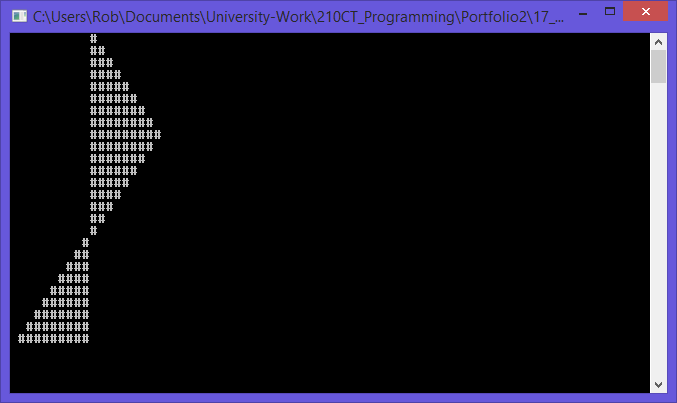
\includegraphics[scale=0.7]{17_Lambda/12.png}
		\end{homeworkSection}
		\pagebreak
		\begin{homeworkSection}{Tasks 3}
			
			\Cscript{17_Lambda/code2}{Wave.cpp Version 2}
			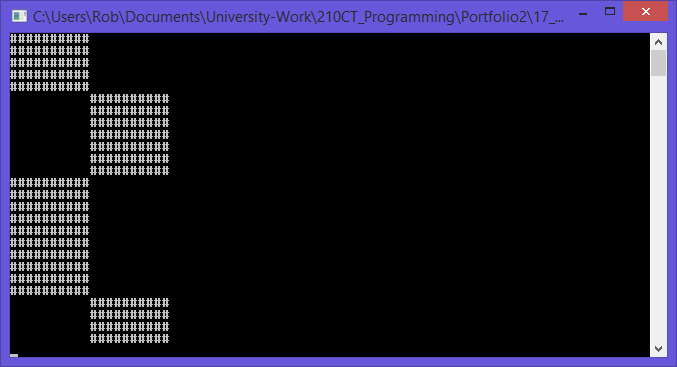
\includegraphics[scale=0.7]{17_Lambda/c2}
		\end{homeworkSection}
		
\end{homeworkProblem}



\end{document}